% nn-5.png -- the 1-hidden-layer, sigmoid network of section 3.5, drawn twice:
%   (a) one input neuron per feature (the honest picture)
%   (b) the same network with the input vector collapsed into one node
% Build: bash tools/figures/build.sh
\documentclass[tikz,border=5pt]{standalone}
% Shared style for the neural-network diagrams in notebooks/img/nn-*.png.
% Palette and look are matched to the pre-existing figures (nn-1..nn-8,
% backprop-*) so a regenerated figure sits next to them unnoticed.
\usepackage[T1]{fontenc}
\usepackage{newtxtext}
\usepackage{newtxmath}
\usetikzlibrary{arrows.meta,calc,positioning}

\definecolor{innavy}{HTML}{004475}     % input neurons, source-like labels
\definecolor{hidyellow}{HTML}{FFCF6E}  % hidden neurons
\definecolor{outmaroon}{HTML}{8E1854}  % output neuron
\definecolor{accgold}{HTML}{E5A600}    % "Hidden Layer" label
\definecolor{gridgrey}{HTML}{B7B7B7}

\tikzset{
  neuron/.style   = {circle, draw=black, line width=0.9pt, minimum size=0.9cm,
                     inner sep=0pt, font=\large\bfseries},
  hidden/.style   = {neuron, fill=hidyellow},
  inputn/.style   = {neuron, fill=innavy, text=white},
  outputn/.style  = {neuron, fill=outmaroon, text=white},
  conn/.style     = {-{Latex[length=2.2mm,width=1.6mm]}, line width=0.7pt},
  bias/.style     = {-{Latex[length=1.8mm,width=1.3mm]}, line width=0.7pt},
  biaslbl/.style  = {font=\scriptsize, inner sep=1pt},
  layerlbl/.style = {font=\large\bfseries},
}

% Column positions shared by every figure (1 unit = 1cm).
\def\HIDX{3.4}   % hidden neurons
\def\ACTX{4.9}   % activation insets (centre)
\def\OUTX{7.4}   % output neuron
\def\NODE{0.45}  % neuron radius
\def\BOX{0.42}   % activation inset half-width

% Framed mini-plot of the sigmoid, drawn where the existing figures draw it.
% Usage: \actinset{x}{y}{label}
\newcommand{\actinset}[3]{%
  \begin{scope}[shift={(#1,#2)}]
    \fill[white] (-\BOX,-\BOX) rectangle (\BOX,\BOX);
    \foreach \g in {-0.14,0.14}{%
      \draw[gridgrey, line width=0.35pt] (-\BOX,\g) -- (\BOX,\g);
      \draw[gridgrey, line width=0.35pt] (\g,-\BOX) -- (\g,\BOX);}
    \draw[black, line width=1.1pt, domain=-0.40:0.40, samples=60]
      plot ({\x}, {0.78/(1+exp(-9*\x)) - 0.39});
    \draw[black, line width=0.9pt] (-\BOX,-\BOX) rectangle (\BOX,\BOX);
    \node[above left, font=\scriptsize, inner sep=1pt] at (\BOX,\BOX+0.02) {#3};
  \end{scope}}

% Bias arrow plus label above a neuron: \biasup{node name}
\newcommand{\biasup}[1]{%
  \draw[bias] ($(#1)+(0,\NODE+0.41)$) -- ($(#1)+(0,\NODE+0.01)$);
  \node[biaslbl, above] at ($(#1)+(0,\NODE+0.41)$) {Bias};}

% A vector collapsed into one node: two offset discs behind it.
% Usage: \vectornode{x}{y}{label}
\newcommand{\vectornode}[3]{%
  \foreach \dx/\dy in {0.13/0.11, 0.26/0.22}{%
    \draw[innavy, line width=0.7pt, fill=innavy!22]
      ($(#1,#2)+(\dx,\dy)$) circle (\NODE);}
  \node[inputn] (#3) at (#1,#2) {$#3$};}

\begin{document}
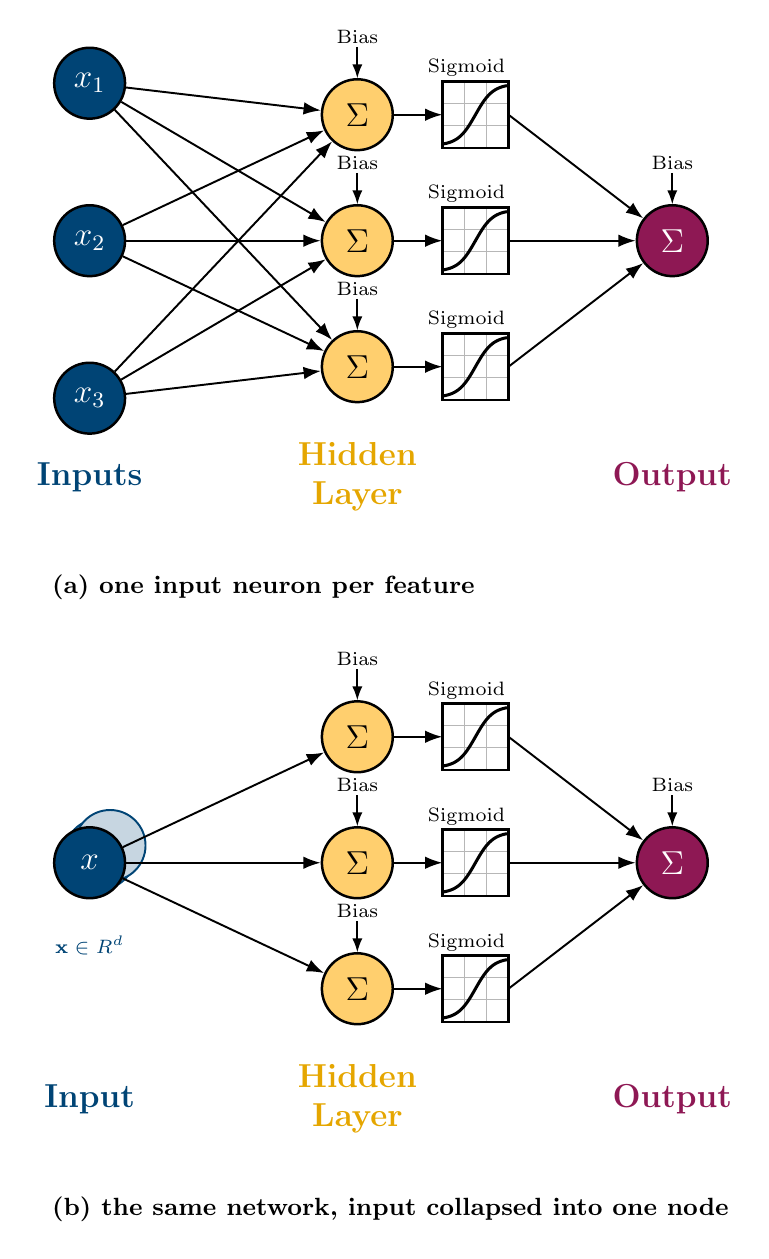
\begin{tikzpicture}[x=1cm,y=1cm]

%---------------------------------------------------------------------
% (a) every feature has its own input neuron
%---------------------------------------------------------------------
\begin{scope}
  \foreach \i/\yy in {1/2.0, 2/0.0, 3/-2.0}{
    \node[inputn] (i\i) at (0,\yy) {$x_{\i}$};}

  \foreach \j/\yy in {1/1.6, 2/0.0, 3/-1.6}{
    \node[hidden] (h\j) at (\HIDX,\yy) {$\Sigma$};
    \actinset{\ACTX}{\yy}{Sigmoid}
    \draw[conn] (h\j) -- (\ACTX-\BOX,\yy);
    \biasup{h\j}}

  \node[outputn] (o1) at (\OUTX,0) {$\Sigma$};
  \biasup{o1}

  \foreach \i in {1,2,3}{\foreach \j in {1,2,3}{%
    \draw[conn] (i\i) -- (h\j);}}
  \foreach \yy in {1.6,0.0,-1.6}{\draw[conn] (\ACTX+\BOX,\yy) -- (o1);}

  \node[layerlbl, text=innavy,    align=center] at (0,-3.0)     {Inputs};
  \node[layerlbl, text=accgold,   align=center] at (\HIDX,-3.0) {Hidden\\Layer};
  \node[layerlbl, text=outmaroon, align=center] at (\OUTX,-3.0) {Output};

  \node[font=\small\bfseries, anchor=west] at (-0.6,-4.4)
    {(a) one input neuron per feature};
\end{scope}

%---------------------------------------------------------------------
% (b) the same network with the input vector collapsed to one node
%---------------------------------------------------------------------
\begin{scope}[yshift=-7.9cm]
  \vectornode{0}{0}{x}

  \foreach \j/\yy in {1/1.6, 2/0.0, 3/-1.6}{
    \node[hidden] (h\j) at (\HIDX,\yy) {$\Sigma$};
    \actinset{\ACTX}{\yy}{Sigmoid}
    \draw[conn] (h\j) -- (\ACTX-\BOX,\yy);
    \biasup{h\j}}

  \node[outputn] (o1) at (\OUTX,0) {$\Sigma$};
  \biasup{o1}

  \foreach \j in {1,2,3}{\draw[conn] (x) -- (h\j);}
  \foreach \yy in {1.6,0.0,-1.6}{\draw[conn] (\ACTX+\BOX,\yy) -- (o1);}

  \node[layerlbl, text=innavy,    align=center] at (0,-3.0)     {Input};
  \node[layerlbl, text=accgold,   align=center] at (\HIDX,-3.0) {Hidden\\Layer};
  \node[layerlbl, text=outmaroon, align=center] at (\OUTX,-3.0) {Output};

  \node[font=\scriptsize, text=innavy] at (0,-1.05) {$\mathbf{x}\in\mathbb{R}^{d}$};

  \node[font=\small\bfseries, anchor=west] at (-0.6,-4.4)
    {(b) the same network, input collapsed into one node};
\end{scope}

\end{tikzpicture}
\end{document}
